\section{D. 시험자리 배정하기}

\begin{frame} % No title at first slide
    \sectiontitle{D}{시험자리 배정하기}
    \sectionmeta{
        \texttt{math, dynamic\_programming, combinatorics}\\
        출제진 의도 -- \textbf{\color{acsilver}Medium}
    }
    \begin{itemize}
        \item 출제자: \texttt{김명기}
    \end{itemize}
\end{frame}

\begin{frame}{\textbf{D}. 시험자리 배정하기}

    \begin{itemize}
    	\item 이 문제는 dp풀이와 조합식을 이용한 풀이가 있습니다.
    	\item 여기에서는 dp풀이를 소개하겠습니다.
    \end{itemize}
    
\end{frame}


\begin{frame}{\textbf{D}. 시험자리 배정하기}
	
	\begin{itemize}
		\item 문제의 정답을 $A(n)$으로 정의하겠습니다.
		\item $A(1) = 1, A(2) = 2$임을 직관적으로 알 수 있습니다.
		\item $k \ge 3$에서$A(k)$의 마지막 자리 2개만 봤을 때 가능한 경우는 아래 3가지 뿐입니다.

	\end{itemize}
	\begin{figure}[h!]
		\centering
		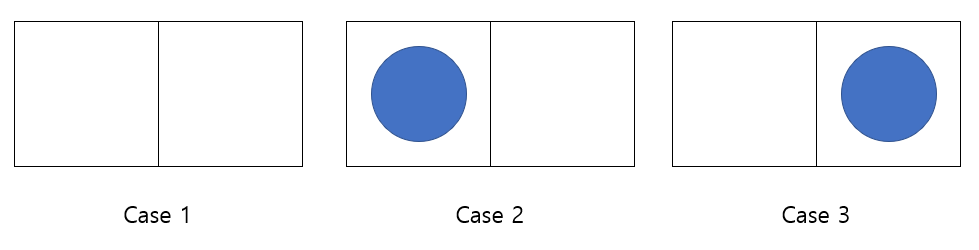
\includegraphics[width=0.7\linewidth]{../images/set-examseats/1.png}
	\end{figure}
\end{frame}

\begin{frame}{\textbf{D}. 시험자리 배정하기}
	\begin{figure}[h!]
		\centering
		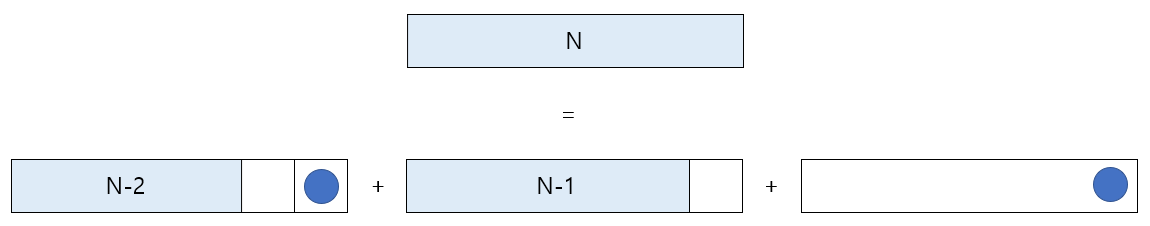
\includegraphics[width=0.9\linewidth]{../images/set-examseats/2.png}
	\end{figure}
	\begin{itemize}

		\item 위와 같이 구성하면 $A(n)$의 모든 경우를 구할 수 있습니다.
		\item 따라서 점화식은 $A(n) = A(n-1) + A(n-2) + 1$이 됩니다.
		\item 총 시간복잡도는 \complexity{n}입니다.
		
	\end{itemize}
	
\end{frame}